\documentclass{article}
\usepackage[utf8]{inputenc}
\usepackage{amsmath}
\usepackage{booktabs}
\usepackage{longtable}
\usepackage{array}
\usepackage{multirow}
\usepackage{xcolor}
\usepackage{hyperref}
\usepackage{geometry}
\geometry{margin=1in}
\usepackage[numbers]{natbib}
\usepackage{placeins}
\usepackage{graphicx}

\title{Supplemental Methods: STATE}
\author{}
\date{}

\begin{document}

\maketitle

\section{STATE}

We benchmarked the State Embedding (``SE'') stage of STATE\cite{adduri2025state}, a self-supervised cell-embedding transformer trained with a tabular optimal-transport-style loss (Wasserstein + energy kernel) over masked gene-expression ``sentences''. Each cell is tokenized into a sequence of (gene, count) pairs, gene tokens are mapped to fixed protein-language-model embeddings, and the sequence is processed by a transformer encoder; a binary decoder simultaneously predicts gene presence to encourage sparse reconstruction.

Following the published recipe, gene tokens are replaced with pretrained protein embeddings from TranscriptFormer\cite{pearce2025transcriptformer}, a cross-species single-cell foundation model. We use the 2{,}560-dimensional gene embeddings released by TranscriptFormer for both \emph{Mus musculus} and \emph{Homo sapiens}, merged into a single multi-species table and matched to each dataset's gene names via Ensembl identifier resolution.

To make STATE comparable to the Geneformer baseline used elsewhere in this study, we override the published SE defaults to a smaller architecture (Table~\ref{tab:state_params}): 256 hidden, 4 attention heads, 3 transformer layers, 512 feed-forward, 256-dim cell-embedding output, dropout 0.02. Because gene tokens are mapped to a fixed embedding table, the trainable parameter count of SE under our configuration is dominated by the encoder, transformer, and decoder ($\sim$3.5--4M trainable parameters across datasets), rather than by a learned gene-vocabulary embedding.

Unlike Geneformer and SCVI, STATE training duration is governed by a fixed \emph{step} budget chosen so that the total amount of optimization remains roughly constant across the sweep, with step-based early stopping (patience $= 5$ validation windows) acting as an upper bound. After training, the best checkpoint is selected by minimum validation loss, and cell embeddings are extracted from this checkpoint for downstream mutual-information estimation.

Figure~\ref{fig:state_training_loss} shows representative training and validation loss curves for SE trained on PBMC at the largest dataset size (46{,}415 cells) and full quality. Both losses decrease monotonically and the validation curve closely tracks training, indicating stable convergence without overfitting.

\begin{figure}[!htbp]
\centering
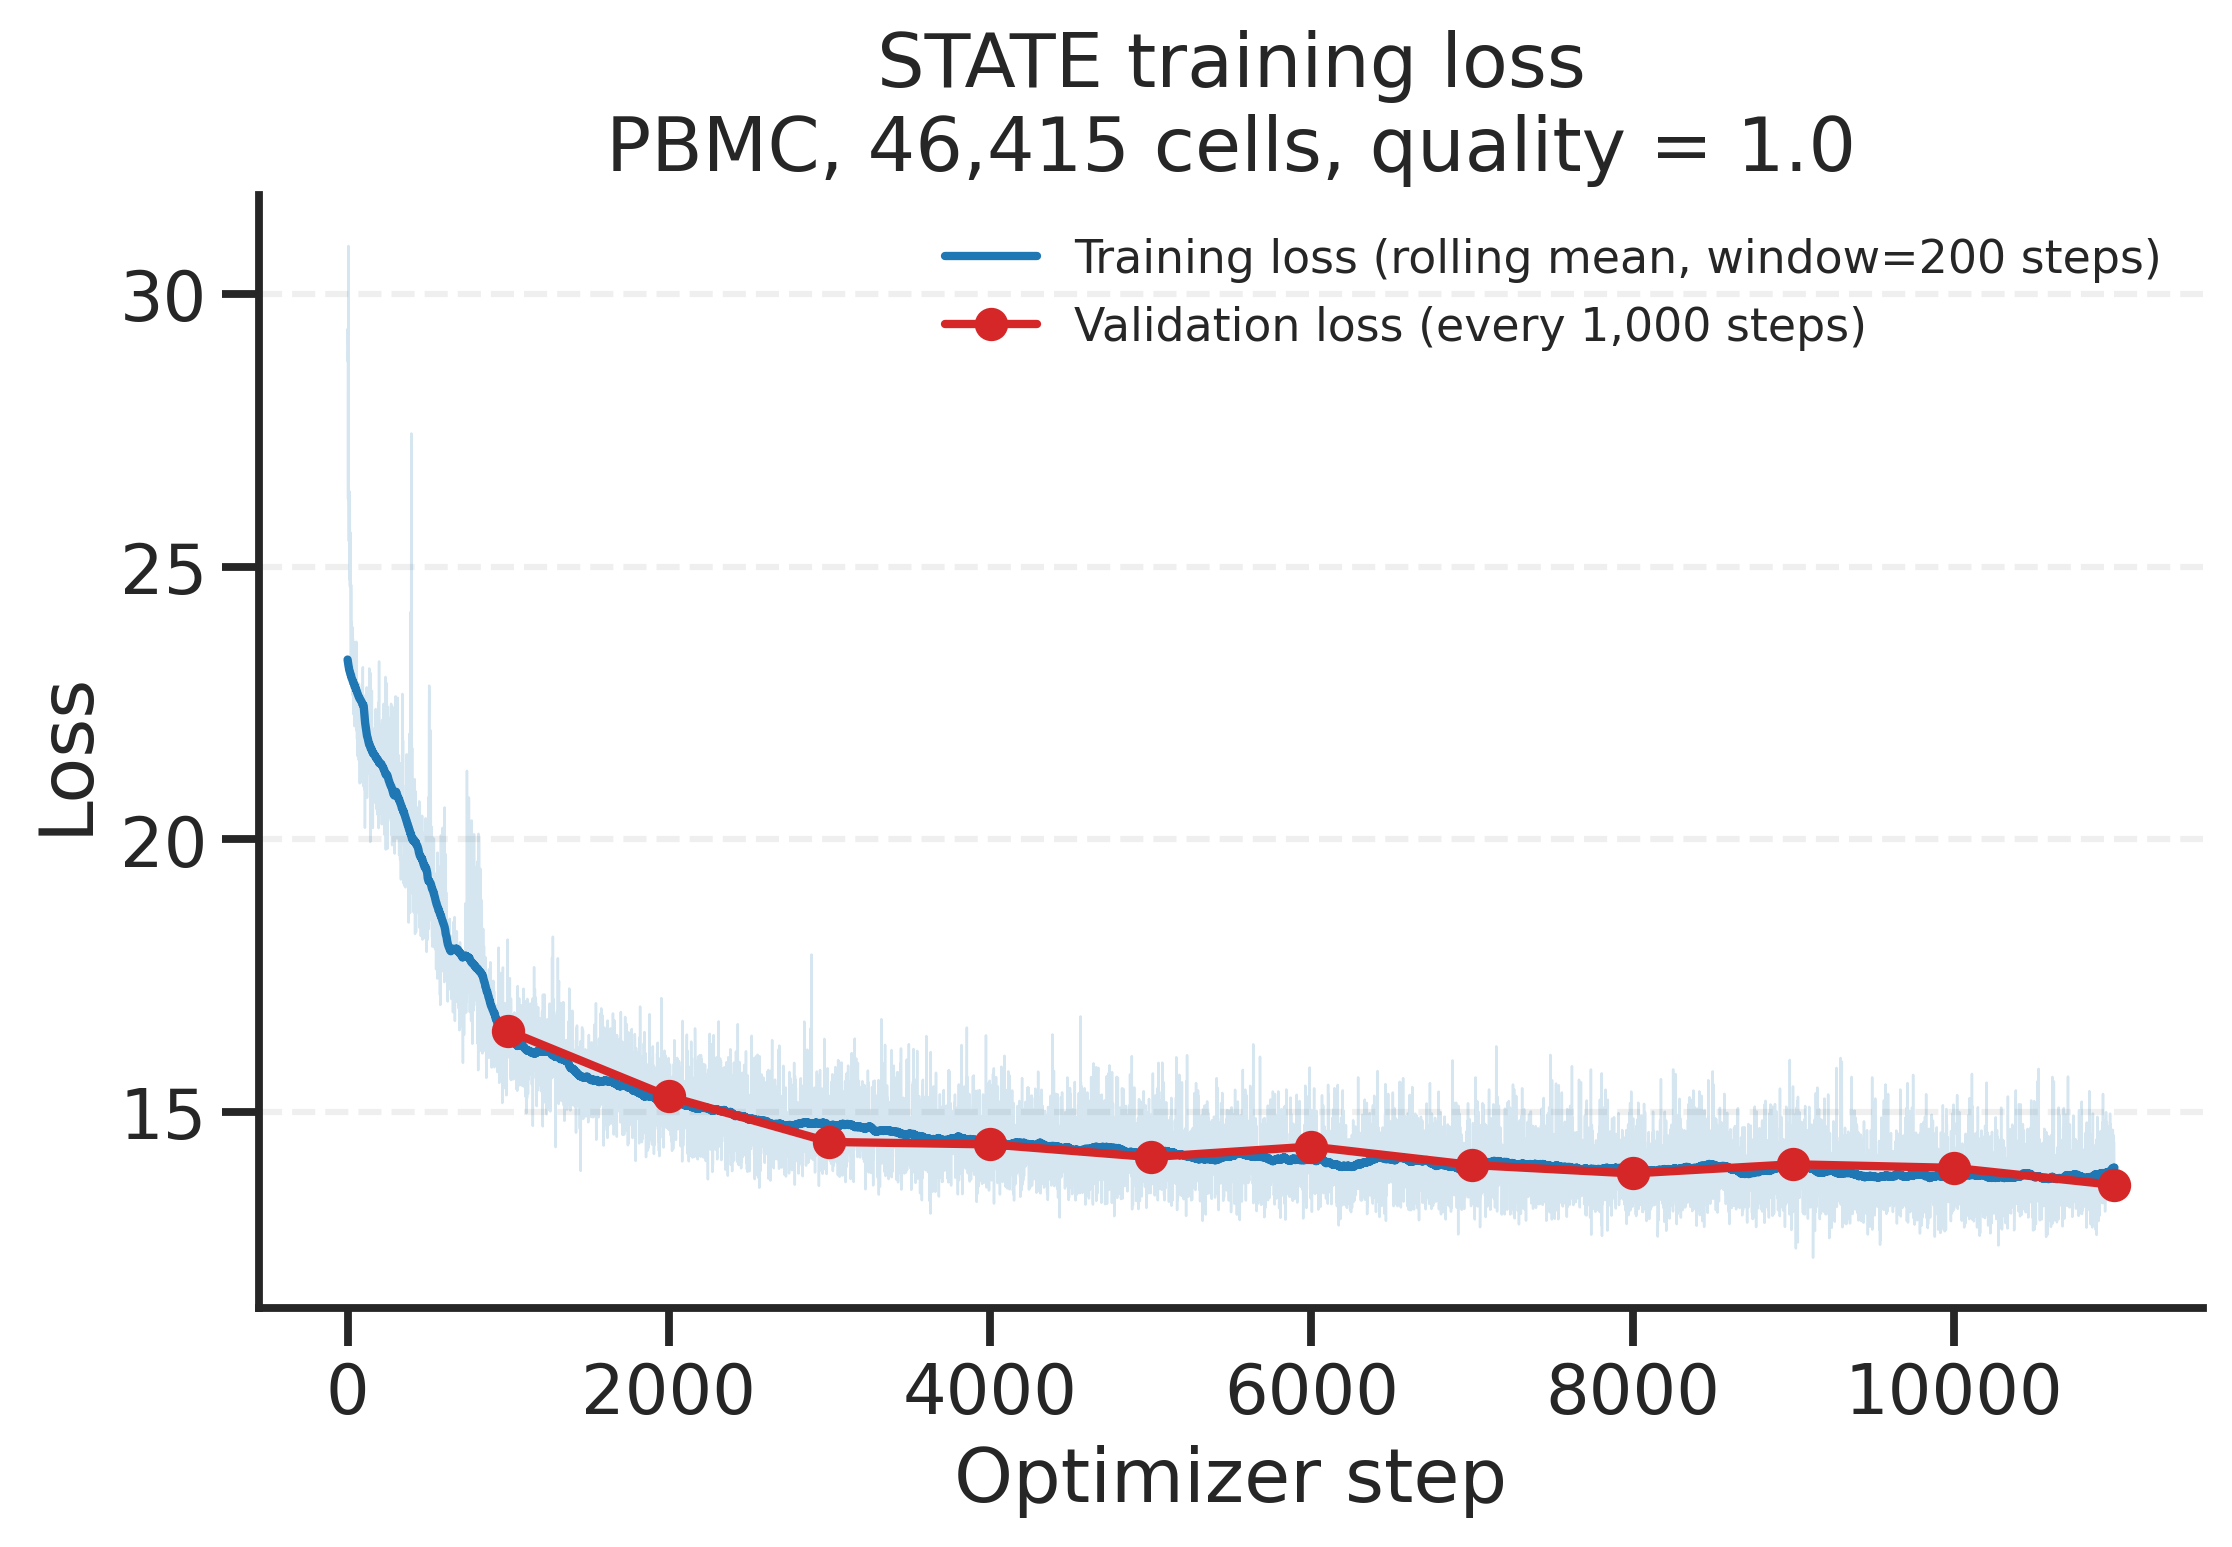
\includegraphics[width=0.8\textwidth]{loss_train_eval_state_pbmc_46k_quality1.png}
\caption{Training and validation loss curves for STATE SE trained on PBMC (46{,}415 cells, quality $=1.0$), shown on linear axes. Validation is computed every 1{,}000 optimizer steps. The raw per-step training loss is plotted faintly in the background, and the bold blue curve overlays a centered rolling mean (window $=$ 200 steps) to suppress minibatch noise; no other smoothing is applied. The validation curve is shown unsmoothed (one point per evaluation).}
\label{fig:state_training_loss}
\end{figure}

\begin{table}[!htbp]
\centering
\caption{Hyperparameters for STATE (SE) as used in this study.}
\label{tab:state_params}
\small
\begin{tabular}{ll}
\toprule
\textbf{Parameter} & \textbf{Value} \\
\midrule
\multicolumn{2}{l}{\textit{Model architecture}} \\
Number of transformer layers & 3 \\
Hidden dimension & 256 \\
Attention heads & 4 \\
Feed-forward dimension & 512 \\
Cell-embedding (output) dimension & 256 \\
Maximum sequence length & 2{,}048 tokens \\
Dropout & 0.02 \\
Gene token embedding & TranscriptFormer protein embeddings (2{,}560-dim, mouse + human) \\
Token-level objective & 20\% variable masking \\
Reconstruction head & Binary gene-presence decoder + count head \\
Loss & Tabular (Wasserstein + energy kernel) \\
\midrule
\multicolumn{2}{l}{\textit{Optimization}} \\
Optimizer & AdamW \\
Maximum learning rate & $1 \times 10^{-4}$ \\
Weight decay & 0.01 \\
Maximum gradient norm & 0.8 \\
Global batch size & 64 \\
LR schedule & OneCycleLR (warmup $0.33$, end $1.0$) \\
\midrule
\multicolumn{2}{l}{\textit{Training and checkpointing}} \\
Validation interval & 1{,}000 optimizer steps \\
Validation batches per check & 50 \\
Best-checkpoint selection & Minimum validation loss \\
Early-stopping patience & 5 validation windows ($\geq 1$-epoch warm-up) \\
\bottomrule
\end{tabular}
\end{table}

\FloatBarrier

\begin{thebibliography}{99}

\bibitem{adduri2025state}
Adduri, A. K., Gautam, D., Bevilacqua, B., Imran, A., Shah, R., Naghipourfar, M., Teyssier, N., Ilango, R., Nagaraj, S., Dong, M., Ricci-Tam, C., Carpenter, C., Subramanyam, V., Winters, A., Tirukkovular, S., Sullivan, J., Plosky, B. S., Eraslan, B., Youngblut, N. D., Leskovec, J., Gilbert, L. A., Konermann, S., Hsu, P. D., Dobin, A., Burke, D. P., Goodarzi, H., \& Roohani, Y. H. (2025). Predicting cellular responses to perturbation across diverse contexts with State. \textit{bioRxiv}. \url{https://www.biorxiv.org/content/10.1101/2025.06.26.661135v2}

\bibitem{pearce2025transcriptformer}
Pearce, J. D., Simmonds, S. E., Mahmoudabadi, G., Krishnan, L., Palla, G., Istrate, A.-M., Tarashansky, A., Nelson, B., Valenzuela, O., Li, D., Quake, S. R., \& Karaletsos, T. (2025). A cross-species generative cell atlas across 1.5 billion years of evolution: the TranscriptFormer single-cell model. \textit{bioRxiv}. \url{https://www.biorxiv.org/content/10.1101/2025.04.25.650731v2}

\bibitem{theodoris2023geneformer}
Theodoris, C. V., Xiao, L., Chopra, A., Chaffin, M. D., Al Sayed, Z. R., Hill, M. C., Mantineo, H., Brydon, E., Zeng, Z., Liu, X. S., \& Ellinor, P. T. (2023). Transfer learning enables predictions in network biology. \textit{Nature}, 618(7965), 616--624.

\end{thebibliography}

\end{document}
